\section{NAO Framework}
\label{sec:03_naoFramework}

As stated\todo{as previously stated}, a complete code framework exists to address the NAO robots' hardware
in C++ by the \ac{SPL} team \textit{HULKs}. \todo{a complete code frame work by the SPL teamHULKs exists to address..}
It is implemented in such manner that \textit{Modules}  \todo{this kinda comes out of the blue.. do you have a flow chart or was this already explained earlier to make this a little more "tangible"} waits for all input
values (\textit{Dependencies}) which are necessary to execute their task.
Modules can be seen as larger coherent operations that perform specific roles.
With the output produced by this Module \todo{ich wuerd das klein schreiben, ist ja kein Eigenname?} (\textit{Productions}), successive
Modules can start to perform their cycle.
Due to this sequential process, modules \todo{musst dich aber entscheiden ob gross oder klein.} are modifiable independently. \todo{for a non-hulks person this whole paragraph seems kinda obscure. Unless you have already explained this earlier, this probably needs some more structred explanation / an accompanying figure}
% -------------------------------------------------------------

The robots are able to communicate wirelessly via \ac{UDP} to operate a as
multi-agent system.
In the team message protocol \todo{team-message protocol}, information about the robot states and
knowledge like the believed ball position is exchanged with team mates.
By the \ac{SPL} rules \cite{rules} they are limited to one team message per
robot per second.
However, for the whistle localization challenge, no particular specification
about the communication was defined \cite{technical_challenge}.
In order to localize the sound source with multiple robots, results of the\todo{eher "Multiple" statt "the". Ansonsten musst du aus "localizations" Singular machen}
single robot whistle localizations are forwarded to the protocol.
% -------------------------------------------------------------

\subsection{Coordinate Systems}
\label{subsec:03_coordinates}

Two coordinate systems are introduced to consider the whistle-sound position \todo{whistle-sound position?}.
One for the relative orientation of the source to the robot's head and another
for the absolute position determination in field coordinates.

\Cref{fig:03_naoCoordinate} visualizes the coordinate system of the
robot.\todo{falsche Referenz zur Section statt zur Figure!!!}
Direction angles $\gamma$ are specified around the z-axis in
mathematically positive direction and range between $-\pi$ and $\pi$.
The direction where the whistle source is believed at by a single robot
will be described as $\gamma$.
% -------------------------------------------------------------

\begin{figure}[ht]
      \centering
      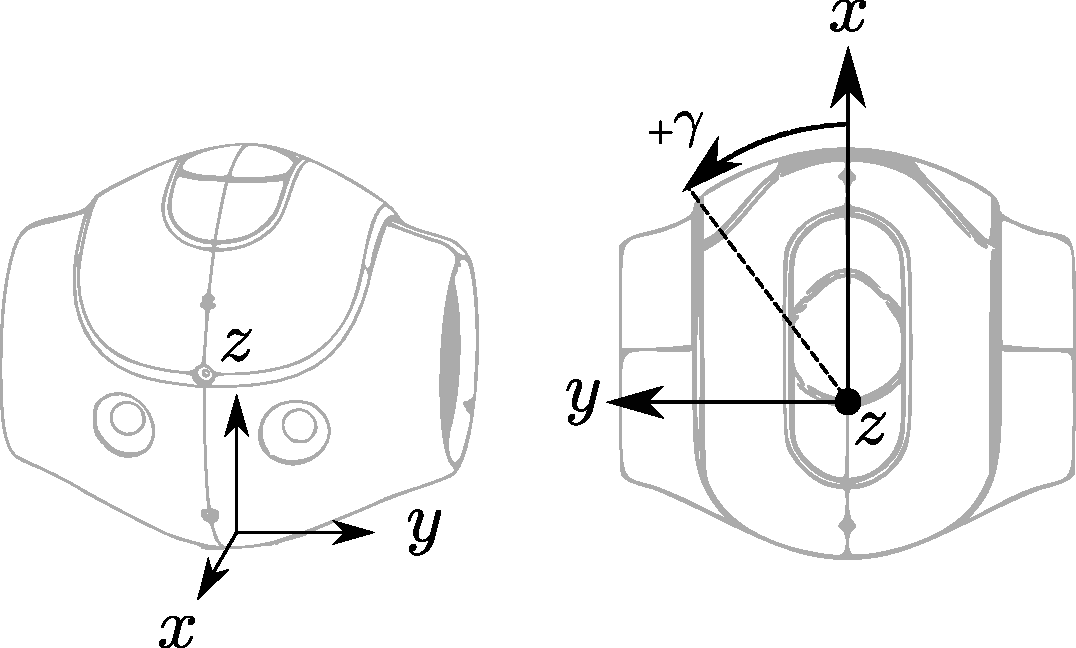
\includegraphics[width=0.60\columnwidth]{figures/nao_coor_both}
      \label{fig:03_naoCoordinate}
      \caption{Coordinate System of NAO's head.}
\end{figure}
% -------------------------------------------------------------

For field coordinates, only the planar case matters in this work.
It is defined as illsutrated in \cref{fig:03_fieldCoordinates}.
In game, the robots play into x-direction.
The whistle position of the team filter will be described
in this coordinate system.
% -------------------------------------------------------------
\begin{figure}[ht]
      \centering
      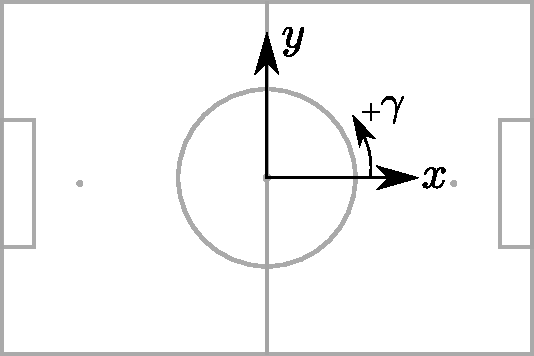
\includegraphics[width=0.50\columnwidth]{figures/field}
      \caption{Field Coordinate System.}
      \label{fig:03_fieldCoordinates}
\end{figure}
% -------------------------------------------------------------

\subsection{Microphones}
\label{subsec:03_microphones}

Four microphones are attached on the NAO's head.
Their positions are listed in \cref{tab:03_micPos} with respect
to the head's coordinate system introduced in \cref{subsec:03_coordinates}
\cite{v6_docu} and outlined in \cref{fig:03_micPos}.
As per documentation \cite{nao_docu}, the operating frequency range
is between 150\si{\hertz} and 12\si{\kilo\hertz}.
The sensitivity is indicated with 20\si{\milli\volt/\pascal\pm3\decibel} at
1\si{\kilo\hertz}.

Prior to this work, there was no need to address more than one microphone
on one \todo{each}robot.
Thus, receiving data from multiple microphone channels was implemented
into the audio interface of the HULKs' framework.
Raw microphone data of all channels is captured in interleaved format
and unpacked by the \lstinline!AudioReceiver! module which makes
the samples accessible per channel for further usage.
The index number of the channels is derived from the order of the
interleaved data format straightforwardly.
The sampling frequency $f_s$ of the microphones is set to 4.1\si{\kilo\hertz}.
% -------------------------------------------------------------
% as \cref{lst:03_buffer} shows.
% \lstinputlisting[float=htp, language=C++, basicstyle=\ttfamily\scriptsize,
%         caption={Deinterleaving procedure of captured microphone data.},
%         label=lst:03_buffer,
%         numbers=left,
%         stepnumber=1]{sourcecodes/audio_capture.cpp}
% -------------------------------------------------------------

% -------------------------------------------------------------

\btline{ht}{1.2}
\btab{|c|c|c|c|}
\hline
Channel & x [\si{\meter}] & y [\si{\meter}] & z [\si{\meter}]\\
\hline
0 & -0.0215 & 0.0558 & 0.0774\\
\hline
1 & -0.0215 & -0.0558 & 0.0774\\
\hline
2 & 0.0206 & 0.0309 & 0.0986\\
\hline
3 & 0.0206 & -0.0309 & 0.0986\\
\hline
\etab
\et{Positions of the microphones on the NAO's head}{03_micPos}
% -------------------------------------------------------------

\begin{figure}[ht]
      \centering
      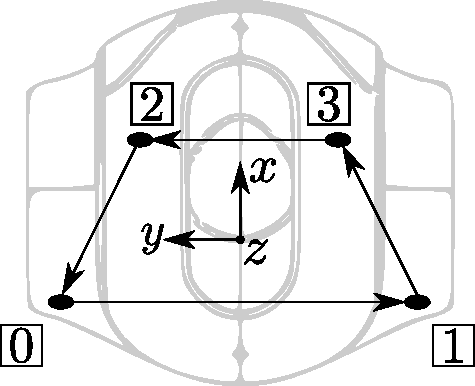
\includegraphics[width=0.35\columnwidth]{figures/mic_pos}
      \caption{Microphone positions on NAO's head.}
      \label{fig:03_micPos}
\end{figure}
% -------------------------------------------------------------

In order to determine the direction of the sound source,
the \ac{TDOA} between two channels is observed in this work.
Hereinafter, the right adjacent channel of the \textit{base channel} is defined as
\textit{next channel}.
This relation is pictured with arrows in \cref{fig:03_micPos} where
the arrowhead points towards the next channel.
From the implementation point of view, this order makes the most sense
when iterating over all channels.

% -------------------------------------------------------------
\btline{ht}{1.2}
\btab{|c|c|}
\hline
Base channel & Next channel\\
\hline
0 & 1 \\
\hline
1 & 3 \\
\hline
2 & 0 \\
\hline
3 & 2 \\
\hline
\etab
\et{Definition of \textbf{next channel} in respect of \textbf{base channel}}{03_channelOrder}
% -------------------------------------------------------------

\subsubsection*{ALSA} \todo{full name in here, no abbrevation}
\label{subsubsec:04_alsa}

Among \todo{"Among" alleine, oder "Along with"}with the addressing of multiple microphones, the audio interface was
reworked and utilizes the open source library \ac{API} of \ac{ALSA} \cite{alsa}.
Using this library, configuration for connecting to the microphones can be realized
as desired.
Here, the \textit{access type} is set to interleaved format.
The data format is set to float 32 bit \todo{das sieht irgendwie komisch aus. Vielleicht irgendwie hervorheben oder anders zusammen schreiben?} as well as the sampling rate to 4.1\si{\kilo\hertz}.
% -------------------------------------------------------------

\subsection{Existing Whistle Detection}
\label{subsec:03_whistleDetection}

Since the whistle detection was already present before this work,
it is introduced only in a short manner.
The existing whistle detection is based on the implementation of the \ac{SPL}
team \ac{UNSW}.
After 1024 samples are collected in the buffer, these samples are Hann-windowed
and then transformed into frequency domain using \ac{FFT}.
A threshold is defined by the mean of the magnitude of the overall spectrum increased
by a factor of 1.3. \todo{A threshold is defined as the mean of the spetrum magnitude, multiplied by a factor of $1.3$}
Dividing the frequency band between 2\si{\kilo\hertz} and 4\si{\kilo\hertz}
into multiple parts, the frequency band is narrowed from both sides until
the mean value of one part exceeds the threshold per side.
If the mean of the remaining frequency band is larger than a second threshold
which is 2.3-fold than the overall mean, a whistle is detected in this frame. \todo{... is larger than 2.5-times the overall mean,...}
Both factors are parameterized.
Whistles need to be detected in multiple \todo{at least two, oder wie viele?} frames within a short period of time \todo{quantify}
until the \lstinline!whistleFound! state is set to true.

For the whistle localization, the boolean of the whistle data can only be set to true
after 3000\si{\milli\second} again. \change[]{better explanation} \todo{YES!}

Only one channel is used for the whistle detection which is channel 0
(rear left) by default. \todo{By default, only channel zero (oder $0$) is used for he whistle detection.}
All transformations into frequency domain are executed with the C++ library
\ac{FFTW}.
This open source library provides most common functions for operations
in frequency domain \todo{... and is widely used?}.
% -------------------------------------------------------------

\subsection{Whistle Localization Structure}
\label{subsec:03_whistleLocalizationStructure}

The procedure of the whistle localization in the context of the existing
NAO framework can be briefly outlined by the following steps:
% -------------------------------------------------------------
\begin{enumerate}
      \item \textbf{Buffer}: the \lstinline!WhistleDirectionEstimation! module saves microphone
            data until whistle is detected by the \lstinline!WhistleDetection! module.
      \item \textbf{Single Robot Whistle Direction Estimation}: \todo{vielleicht mit Bindestrichen etwas uebersichtlicher: Single-robot whistle-direction estimation ode so aehnlich} the \lstinline!WhistleDirectionEstimation!
            performs the sound source localization algorithm and outputs a
            believed direction angle and additional information if a whistle was detected.
            The signal start detection is part of this module.
      \item \textbf{Send Direction via Team Message}: angular direction result plus additional information
            are sent to other robots by team message.
      \item \textbf{Multi-Agent Whistle Localization}: wait for results of all agents to be present
            and filter direction information for a final sound position.
\end{enumerate}
% -------------------------------------------------------------